% Generated from audited follow-up artifacts. Do not hand-edit numbers.
\section{Matched Assignment Study: Complete Results}\label{app:furesults}
\begin{table*}[t]
\nolinenumbers
\centering
\small
\setlength{\tabcolsep}{3pt}
\begin{tabular}{lrrrrr}
\toprule
Rate & Comparator & $\Delta$ I$\to$T & 99.7222\% interval & $\Delta$ T$\to$I & 99.7222\% interval\\
\midrule
$10^{-4}$ & Source & -6.000 & $[-9.037,-3.063]$ & +0.120 & $[-1.087,+1.322]$\\
$10^{-4}$ & Count & -0.978 & $[-3.389,+1.379]$ & +1.811 & $[+0.631,+2.995]$\\
$10^{-4}$ & Strata & -0.744 & $[-3.001,+1.436]$ & +1.540 & $[+0.504,+2.583]$\\
$3\cdot10^{-4}$ & Source & -7.133 & $[-10.367,-3.796]$ & -1.320 & $[-2.955,+0.381]$\\
$3\cdot10^{-4}$ & Count & +1.322 & $[-1.730,+4.114]$ & +4.838 & $[+3.332,+6.376]$\\
$3\cdot10^{-4}$ & Strata & +0.122 & $[-2.659,+2.815]$ & +3.820 & $[+2.412,+5.198]$\\
$10^{-3}$ & Source & -10.833 & $[-14.341,-7.330]$ & -1.900 & $[-3.962,+0.148]$\\
$10^{-3}$ & Count & +3.789 & $[+0.717,+6.922]$ & +7.038 & $[+5.163,+8.832]$\\
$10^{-3}$ & Strata & +0.222 & $[-2.591,+3.025]$ & +4.084 & $[+2.426,+5.804]$\\
\bottomrule
\end{tabular}
\caption{All 18 primary effects. Differences are supported minus comparator, in percentage points. Randomized comparators average all three assignment draws within each training seed before seed averaging. Intervals resample images and condition on the fitted seeds and draws.}\label{tab:fuprimary}
\end{table*}
\subsection{Every terminal draw and training seed}
Each row below is one epoch-ten fit. Count and Strata numbers identify assignment draws; no draw is selected for reporting. All entries are percentages.
\begin{table*}[t]
\nolinenumbers
\centering
\small
\setlength{\tabcolsep}{3pt}
\begin{tabular}{lrrrrrrrrr}
\toprule
Policy & Rate & Seed & Rel. & Edited & Both & e I$\to$T & e T$\to$I & C I$\to$T & C T$\to$I\\
\midrule
Source & $10^{-4}$ & 17 & 77.99 & 81.01 & 63.93 & 84.90 & 65.74 & 53.98 & 36.95\\
Source & $10^{-4}$ & 29 & 77.62 & 80.93 & 64.31 & 84.60 & 66.12 & 53.82 & 36.97\\
Source & $10^{-4}$ & 43 & 77.65 & 81.04 & 64.39 & 84.60 & 66.06 & 53.52 & 36.97\\
Source & $3\cdot10^{-4}$ & 17 & 75.23 & 80.22 & 63.65 & 80.20 & 62.62 & 50.56 & 34.36\\
Source & $3\cdot10^{-4}$ & 29 & 75.62 & 79.96 & 63.61 & 82.30 & 63.00 & 50.74 & 34.63\\
Source & $3\cdot10^{-4}$ & 43 & 75.21 & 80.26 & 64.05 & 82.10 & 63.32 & 50.82 & 34.61\\
Source & $10^{-3}$ & 17 & 69.88 & 76.35 & 59.34 & 76.30 & 52.72 & 43.42 & 26.28\\
Source & $10^{-3}$ & 29 & 71.52 & 76.93 & 60.33 & 75.90 & 54.88 & 43.68 & 26.70\\
Source & $10^{-3}$ & 43 & 70.12 & 75.76 & 61.07 & 75.70 & 54.72 & 43.84 & 26.79\\
Supported & $10^{-4}$ & 17 & 87.64 & 83.96 & 67.90 & 78.40 & 65.96 & 49.02 & 36.54\\
Supported & $10^{-4}$ & 29 & 87.69 & 84.01 & 67.71 & 79.10 & 66.14 & 48.96 & 36.41\\
Supported & $10^{-4}$ & 43 & 87.52 & 83.84 & 67.63 & 78.60 & 66.18 & 49.16 & 36.35\\
Supported & $3\cdot10^{-4}$ & 17 & 86.54 & 83.26 & 66.93 & 74.90 & 61.08 & 45.06 & 33.38\\
Supported & $3\cdot10^{-4}$ & 29 & 86.79 & 83.54 & 66.91 & 74.40 & 62.16 & 45.24 & 33.82\\
Supported & $3\cdot10^{-4}$ & 43 & 86.71 & 83.25 & 67.63 & 73.90 & 61.74 & 43.46 & 33.70\\
Supported & $10^{-3}$ & 17 & 85.82 & 81.47 & 65.21 & 65.20 & 51.34 & 36.44 & 25.97\\
Supported & $10^{-3}$ & 29 & 85.90 & 81.33 & 65.38 & 65.70 & 52.96 & 37.40 & 26.62\\
Supported & $10^{-3}$ & 43 & 85.61 & 81.04 & 66.26 & 64.50 & 52.32 & 35.46 & 26.94\\
\bottomrule
\end{tabular}
\caption{Terminal per-seed results. e denotes the full e-ViL source-caption pool and C denotes COCO. Other endpoints follow Table~\ref{tab:secondary}.}\label{tab:futerm0}
\end{table*}
\begin{table*}[t]
\nolinenumbers
\centering
\small
\setlength{\tabcolsep}{3pt}
\begin{tabular}{lrrrrrrrrr}
\toprule
Policy & Rate & Seed & Rel. & Edited & Both & e I$\to$T & e T$\to$I & C I$\to$T & C T$\to$I\\
\midrule
Count 1 & $10^{-4}$ & 17 & 79.20 & 82.53 & 65.21 & 79.20 & 64.14 & 49.76 & 35.73\\
Count 1 & $10^{-4}$ & 29 & 78.99 & 82.52 & 65.19 & 79.40 & 64.56 & 50.54 & 35.82\\
Count 1 & $10^{-4}$ & 43 & 79.38 & 82.96 & 65.52 & 80.10 & 64.54 & 50.54 & 35.64\\
Count 1 & $3\cdot10^{-4}$ & 17 & 76.45 & 80.55 & 63.19 & 72.10 & 56.52 & 44.30 & 31.06\\
Count 1 & $3\cdot10^{-4}$ & 29 & 76.87 & 80.67 & 63.61 & 72.40 & 56.28 & 44.32 & 30.74\\
Count 1 & $3\cdot10^{-4}$ & 43 & 75.85 & 79.79 & 63.63 & 73.30 & 56.54 & 44.04 & 30.42\\
Count 1 & $10^{-3}$ & 17 & 74.92 & 77.82 & 59.81 & 61.20 & 45.12 & 34.88 & 22.57\\
Count 1 & $10^{-3}$ & 29 & 74.66 & 78.15 & 61.57 & 60.00 & 43.60 & 33.94 & 22.14\\
Count 1 & $10^{-3}$ & 43 & 73.58 & 77.41 & 60.04 & 63.70 & 43.96 & 34.80 & 22.04\\
Count 2 & $10^{-4}$ & 17 & 78.90 & 82.89 & 64.91 & 79.90 & 63.98 & 49.76 & 35.55\\
Count 2 & $10^{-4}$ & 29 & 79.07 & 82.76 & 65.65 & 78.30 & 64.52 & 49.82 & 35.47\\
Count 2 & $10^{-4}$ & 43 & 79.20 & 82.93 & 65.15 & 79.70 & 64.28 & 50.12 & 35.48\\
Count 2 & $3\cdot10^{-4}$ & 17 & 77.19 & 81.19 & 63.28 & 72.10 & 56.84 & 44.10 & 30.64\\
Count 2 & $3\cdot10^{-4}$ & 29 & 75.93 & 81.05 & 63.55 & 73.40 & 56.66 & 44.22 & 30.56\\
Count 2 & $3\cdot10^{-4}$ & 43 & 75.02 & 80.36 & 62.88 & 72.80 & 56.84 & 45.12 & 30.17\\
Count 2 & $10^{-3}$ & 17 & 73.68 & 76.93 & 60.35 & 59.00 & 44.36 & 33.36 & 22.26\\
Count 2 & $10^{-3}$ & 29 & 74.34 & 77.58 & 60.84 & 62.10 & 45.24 & 34.92 & 22.74\\
Count 2 & $10^{-3}$ & 43 & 74.51 & 78.22 & 60.67 & 61.60 & 45.22 & 33.60 & 22.54\\
\bottomrule
\end{tabular}
\caption{Terminal per-seed results. e denotes the full e-ViL source-caption pool and C denotes COCO. Other endpoints follow Table~\ref{tab:secondary}.}\label{tab:futerm1}
\end{table*}
\begin{table*}[t]
\nolinenumbers
\centering
\small
\setlength{\tabcolsep}{3pt}
\begin{tabular}{lrrrrrrrrr}
\toprule
Policy & Rate & Seed & Rel. & Edited & Both & e I$\to$T & e T$\to$I & C I$\to$T & C T$\to$I\\
\midrule
Count 3 & $10^{-4}$ & 17 & 79.26 & 82.65 & 64.98 & 79.80 & 64.18 & 49.98 & 35.15\\
Count 3 & $10^{-4}$ & 29 & 78.75 & 82.45 & 64.98 & 80.60 & 64.14 & 50.18 & 35.14\\
Count 3 & $10^{-4}$ & 43 & 79.05 & 82.61 & 64.83 & 80.10 & 64.20 & 50.14 & 35.29\\
Count 3 & $3\cdot10^{-4}$ & 17 & 76.63 & 80.89 & 63.80 & 73.40 & 57.28 & 43.80 & 30.99\\
Count 3 & $3\cdot10^{-4}$ & 29 & 75.82 & 80.69 & 63.53 & 74.00 & 56.96 & 44.18 & 30.59\\
Count 3 & $3\cdot10^{-4}$ & 43 & 75.63 & 80.12 & 63.13 & 74.20 & 57.48 & 44.52 & 30.74\\
Count 3 & $10^{-3}$ & 17 & 74.08 & 77.11 & 59.87 & 61.70 & 46.16 & 34.00 & 22.62\\
Count 3 & $10^{-3}$ & 29 & 73.55 & 76.95 & 60.29 & 61.90 & 46.86 & 34.48 & 21.77\\
Count 3 & $10^{-3}$ & 43 & 72.76 & 77.38 & 60.58 & 60.90 & 46.00 & 33.82 & 21.76\\
Strata 1 & $10^{-4}$ & 17 & 81.51 & 82.80 & 65.82 & 78.90 & 64.44 & 50.18 & 35.71\\
Strata 1 & $10^{-4}$ & 29 & 81.36 & 82.95 & 66.03 & 78.90 & 64.52 & 50.42 & 35.82\\
Strata 1 & $10^{-4}$ & 43 & 80.98 & 82.98 & 65.92 & 78.90 & 64.64 & 49.88 & 35.70\\
Strata 1 & $3\cdot10^{-4}$ & 17 & 78.88 & 81.47 & 63.88 & 74.00 & 57.64 & 45.44 & 31.31\\
Strata 1 & $3\cdot10^{-4}$ & 29 & 78.19 & 81.15 & 63.95 & 72.30 & 58.22 & 45.42 & 31.26\\
Strata 1 & $3\cdot10^{-4}$ & 43 & 78.24 & 81.07 & 64.70 & 74.10 & 58.52 & 45.46 & 31.38\\
Strata 1 & $10^{-3}$ & 17 & 76.90 & 79.23 & 62.94 & 65.20 & 45.86 & 36.06 & 23.48\\
Strata 1 & $10^{-3}$ & 29 & 76.16 & 77.50 & 62.10 & 63.70 & 49.74 & 37.00 & 24.13\\
Strata 1 & $10^{-3}$ & 43 & 75.27 & 79.34 & 62.06 & 63.50 & 47.22 & 35.84 & 23.41\\
\bottomrule
\end{tabular}
\caption{Terminal per-seed results. e denotes the full e-ViL source-caption pool and C denotes COCO. Other endpoints follow Table~\ref{tab:secondary}.}\label{tab:futerm2}
\end{table*}
\begin{table*}[t]
\nolinenumbers
\centering
\small
\setlength{\tabcolsep}{3pt}
\begin{tabular}{lrrrrrrrrr}
\toprule
Policy & Rate & Seed & Rel. & Edited & Both & e I$\to$T & e T$\to$I & C I$\to$T & C T$\to$I\\
\midrule
Strata 2 & $10^{-4}$ & 17 & 80.71 & 83.17 & 65.84 & 79.90 & 64.72 & 50.30 & 35.74\\
Strata 2 & $10^{-4}$ & 29 & 81.00 & 83.06 & 66.47 & 79.50 & 64.78 & 50.14 & 35.74\\
Strata 2 & $10^{-4}$ & 43 & 80.49 & 83.53 & 66.07 & 80.10 & 64.46 & 49.80 & 35.65\\
Strata 2 & $3\cdot10^{-4}$ & 17 & 78.51 & 82.71 & 65.55 & 73.60 & 57.72 & 44.82 & 31.58\\
Strata 2 & $3\cdot10^{-4}$ & 29 & 78.18 & 82.01 & 65.21 & 75.30 & 57.18 & 45.66 & 31.54\\
Strata 2 & $3\cdot10^{-4}$ & 43 & 77.73 & 81.85 & 65.10 & 73.80 & 58.58 & 45.62 & 31.52\\
Strata 2 & $10^{-3}$ & 17 & 76.49 & 79.10 & 62.73 & 64.80 & 47.82 & 36.80 & 23.46\\
Strata 2 & $10^{-3}$ & 29 & 75.84 & 79.55 & 62.37 & 66.70 & 49.52 & 38.30 & 23.83\\
Strata 2 & $10^{-3}$ & 43 & 76.65 & 79.56 & 62.98 & 65.20 & 48.40 & 37.00 & 24.16\\
Strata 3 & $10^{-4}$ & 17 & 81.49 & 82.64 & 65.38 & 79.40 & 64.54 & 50.10 & 35.50\\
Strata 3 & $10^{-4}$ & 29 & 81.24 & 82.93 & 65.57 & 79.90 & 64.54 & 50.14 & 35.62\\
Strata 3 & $10^{-4}$ & 43 & 81.38 & 82.95 & 65.76 & 79.50 & 64.34 & 49.88 & 35.46\\
Strata 3 & $3\cdot10^{-4}$ & 17 & 78.48 & 81.51 & 63.53 & 74.80 & 57.60 & 45.50 & 31.18\\
Strata 3 & $3\cdot10^{-4}$ & 29 & 78.14 & 81.25 & 63.72 & 74.30 & 57.64 & 45.82 & 30.96\\
Strata 3 & $3\cdot10^{-4}$ & 43 & 78.60 & 81.43 & 63.72 & 76.30 & 57.46 & 45.68 & 31.30\\
Strata 3 & $10^{-3}$ & 17 & 76.59 & 79.06 & 61.05 & 63.70 & 47.60 & 36.26 & 23.56\\
Strata 3 & $10^{-3}$ & 29 & 76.18 & 77.95 & 62.10 & 66.30 & 48.70 & 37.30 & 23.81\\
Strata 3 & $10^{-3}$ & 43 & 76.86 & 79.11 & 62.14 & 65.10 & 48.24 & 35.02 & 24.02\\
\bottomrule
\end{tabular}
\caption{Terminal per-seed results. e denotes the full e-ViL source-caption pool and C denotes COCO. Other endpoints follow Table~\ref{tab:secondary}.}\label{tab:futerm3}
\end{table*}
\subsection{Both complete selection strategies}
\begin{table*}[t]
\nolinenumbers
\centering
\small
\setlength{\tabcolsep}{3pt}
\begin{tabular}{lrrrrrrrrrr}
\toprule
Selector & Policy & Seed & Ep. & Rel. & Edited & Both & e I$\to$T & e T$\to$I & C I$\to$T & C T$\to$I\\
\midrule
Native & Source & 17 & 1 & 81.35 & 83.44 & 67.65 & 84.90 & 69.68 & 56.28 & 39.65\\
Native & Source & 29 & 1 & 81.09 & 83.42 & 68.09 & 85.00 & 69.74 & 56.02 & 39.46\\
Native & Source & 43 & 3 & 81.12 & 82.91 & 66.47 & 84.20 & 68.64 & 55.26 & 39.02\\
Native & Supported & 17 & 5 & 86.75 & 83.38 & 67.58 & 78.20 & 63.62 & 48.36 & 35.40\\
Native & Supported & 29 & 10 & 86.79 & 83.54 & 66.91 & 74.40 & 62.16 & 45.24 & 33.82\\
Native & Supported & 43 & 5 & 87.46 & 83.25 & 67.19 & 78.40 & 64.12 & 48.28 & 35.30\\
Native & Count 1 & 17 & 0 & 79.47 & 81.21 & 68.95 & 84.50 & 69.76 & 56.32 & 39.35\\
Native & Count 1 & 29 & 0 & 79.47 & 81.21 & 68.95 & 84.50 & 69.76 & 56.32 & 39.35\\
Native & Count 1 & 43 & 0 & 79.47 & 81.21 & 68.95 & 84.50 & 69.76 & 56.32 & 39.35\\
Native & Count 2 & 17 & 0 & 79.47 & 81.21 & 68.95 & 84.50 & 69.76 & 56.32 & 39.35\\
Native & Count 2 & 29 & 0 & 79.47 & 81.21 & 68.95 & 84.50 & 69.76 & 56.32 & 39.35\\
Native & Count 2 & 43 & 0 & 79.47 & 81.21 & 68.95 & 84.50 & 69.76 & 56.32 & 39.35\\
Native & Count 3 & 17 & 0 & 79.47 & 81.21 & 68.95 & 84.50 & 69.76 & 56.32 & 39.35\\
Native & Count 3 & 29 & 0 & 79.47 & 81.21 & 68.95 & 84.50 & 69.76 & 56.32 & 39.35\\
Native & Count 3 & 43 & 0 & 79.47 & 81.21 & 68.95 & 84.50 & 69.76 & 56.32 & 39.35\\
Native & Strata 1 & 17 & 0 & 79.47 & 81.21 & 68.95 & 84.50 & 69.76 & 56.32 & 39.35\\
\bottomrule
\end{tabular}
\caption{Every selected training-seed state. Each random draw has its own learning-rate and epoch selection; there is no winning-draw search. The source manifest records exact state IDs and learning rates.}\label{tab:fusel0}
\end{table*}
\begin{table*}[t]
\nolinenumbers
\centering
\small
\setlength{\tabcolsep}{3pt}
\begin{tabular}{lrrrrrrrrrr}
\toprule
Selector & Policy & Seed & Ep. & Rel. & Edited & Both & e I$\to$T & e T$\to$I & C I$\to$T & C T$\to$I\\
\midrule
Native & Strata 1 & 29 & 0 & 79.47 & 81.21 & 68.95 & 84.50 & 69.76 & 56.32 & 39.35\\
Native & Strata 1 & 43 & 0 & 79.47 & 81.21 & 68.95 & 84.50 & 69.76 & 56.32 & 39.35\\
Native & Strata 2 & 17 & 0 & 79.47 & 81.21 & 68.95 & 84.50 & 69.76 & 56.32 & 39.35\\
Native & Strata 2 & 29 & 0 & 79.47 & 81.21 & 68.95 & 84.50 & 69.76 & 56.32 & 39.35\\
Native & Strata 2 & 43 & 0 & 79.47 & 81.21 & 68.95 & 84.50 & 69.76 & 56.32 & 39.35\\
Native & Strata 3 & 17 & 7 & 80.11 & 82.09 & 65.00 & 78.30 & 60.84 & 48.36 & 33.71\\
Native & Strata 3 & 29 & 0 & 79.47 & 81.21 & 68.95 & 84.50 & 69.76 & 56.32 & 39.35\\
Native & Strata 3 & 43 & 0 & 79.47 & 81.21 & 68.95 & 84.50 & 69.76 & 56.32 & 39.35\\
Retrieval & Source & 17 & 1 & 81.35 & 83.44 & 67.65 & 84.90 & 69.68 & 56.28 & 39.65\\
Retrieval & Source & 29 & 2 & 80.96 & 83.29 & 67.06 & 84.90 & 69.64 & 56.04 & 39.60\\
Retrieval & Source & 43 & 2 & 81.15 & 83.14 & 67.08 & 84.70 & 69.78 & 55.94 & 39.40\\
Retrieval & Supported & 17 & 0 & 79.47 & 81.21 & 68.95 & 84.50 & 69.76 & 56.32 & 39.35\\
Retrieval & Supported & 29 & 0 & 79.47 & 81.21 & 68.95 & 84.50 & 69.76 & 56.32 & 39.35\\
Retrieval & Supported & 43 & 0 & 79.47 & 81.21 & 68.95 & 84.50 & 69.76 & 56.32 & 39.35\\
Retrieval & Count 1 & 17 & 0 & 79.47 & 81.21 & 68.95 & 84.50 & 69.76 & 56.32 & 39.35\\
Retrieval & Count 1 & 29 & 0 & 79.47 & 81.21 & 68.95 & 84.50 & 69.76 & 56.32 & 39.35\\
\bottomrule
\end{tabular}
\caption{Every selected training-seed state. Each random draw has its own learning-rate and epoch selection; there is no winning-draw search. The source manifest records exact state IDs and learning rates.}\label{tab:fusel1}
\end{table*}
\begin{table*}[t]
\nolinenumbers
\centering
\small
\setlength{\tabcolsep}{3pt}
\begin{tabular}{lrrrrrrrrrr}
\toprule
Selector & Policy & Seed & Ep. & Rel. & Edited & Both & e I$\to$T & e T$\to$I & C I$\to$T & C T$\to$I\\
\midrule
Retrieval & Count 1 & 43 & 0 & 79.47 & 81.21 & 68.95 & 84.50 & 69.76 & 56.32 & 39.35\\
Retrieval & Count 2 & 17 & 0 & 79.47 & 81.21 & 68.95 & 84.50 & 69.76 & 56.32 & 39.35\\
Retrieval & Count 2 & 29 & 0 & 79.47 & 81.21 & 68.95 & 84.50 & 69.76 & 56.32 & 39.35\\
Retrieval & Count 2 & 43 & 0 & 79.47 & 81.21 & 68.95 & 84.50 & 69.76 & 56.32 & 39.35\\
Retrieval & Count 3 & 17 & 0 & 79.47 & 81.21 & 68.95 & 84.50 & 69.76 & 56.32 & 39.35\\
Retrieval & Count 3 & 29 & 0 & 79.47 & 81.21 & 68.95 & 84.50 & 69.76 & 56.32 & 39.35\\
Retrieval & Count 3 & 43 & 0 & 79.47 & 81.21 & 68.95 & 84.50 & 69.76 & 56.32 & 39.35\\
Retrieval & Strata 1 & 17 & 0 & 79.47 & 81.21 & 68.95 & 84.50 & 69.76 & 56.32 & 39.35\\
Retrieval & Strata 1 & 29 & 0 & 79.47 & 81.21 & 68.95 & 84.50 & 69.76 & 56.32 & 39.35\\
Retrieval & Strata 1 & 43 & 0 & 79.47 & 81.21 & 68.95 & 84.50 & 69.76 & 56.32 & 39.35\\
Retrieval & Strata 2 & 17 & 0 & 79.47 & 81.21 & 68.95 & 84.50 & 69.76 & 56.32 & 39.35\\
Retrieval & Strata 2 & 29 & 0 & 79.47 & 81.21 & 68.95 & 84.50 & 69.76 & 56.32 & 39.35\\
Retrieval & Strata 2 & 43 & 0 & 79.47 & 81.21 & 68.95 & 84.50 & 69.76 & 56.32 & 39.35\\
Retrieval & Strata 3 & 17 & 0 & 79.47 & 81.21 & 68.95 & 84.50 & 69.76 & 56.32 & 39.35\\
Retrieval & Strata 3 & 29 & 0 & 79.47 & 81.21 & 68.95 & 84.50 & 69.76 & 56.32 & 39.35\\
Retrieval & Strata 3 & 43 & 0 & 79.47 & 81.21 & 68.95 & 84.50 & 69.76 & 56.32 & 39.35\\
\bottomrule
\end{tabular}
\caption{Every selected training-seed state. Each random draw has its own learning-rate and epoch selection; there is no winning-draw search. The source manifest records exact state IDs and learning rates.}\label{tab:fusel2}
\end{table*}
\subsection{Complete descriptive trajectory means}
\begin{table*}[t]
\nolinenumbers
\centering
\small
\setlength{\tabcolsep}{3pt}
\begin{tabular}{lrrrrrrrrr}
\toprule
Policy & Rate & Ep. & Rel. & Edited & Both & First & Alternative & e I$\to$T & e T$\to$I\\
\midrule
Source & $10^{-4}$ & 1 & 81.23 & 83.40 & 67.94 & 80.95 & 73.10 & 84.77 & 69.81\\
Source & $10^{-4}$ & 5 & 80.07 & 81.89 & 65.55 & 80.16 & 70.25 & 84.13 & 67.89\\
Source & $10^{-4}$ & 10 & 77.75 & 81.00 & 64.21 & 80.16 & 68.78 & 84.70 & 65.97\\
Source & $3\cdot10^{-4}$ & 1 & 80.63 & 82.32 & 65.48 & 80.22 & 70.38 & 83.00 & 67.57\\
Source & $3\cdot10^{-4}$ & 5 & 76.53 & 80.17 & 63.55 & 79.41 & 68.38 & 82.60 & 64.24\\
Source & $3\cdot10^{-4}$ & 10 & 75.35 & 80.14 & 63.77 & 79.22 & 68.63 & 81.53 & 62.98\\
Source & $10^{-3}$ & 1 & 74.94 & 77.38 & 61.03 & 77.34 & 65.76 & 74.07 & 50.36\\
Source & $10^{-3}$ & 5 & 73.25 & 77.57 & 61.71 & 77.35 & 67.05 & 75.53 & 54.15\\
Source & $10^{-3}$ & 10 & 70.51 & 76.35 & 60.25 & 76.59 & 65.51 & 75.97 & 54.11\\
Supported & $10^{-4}$ & 1 & 86.72 & 85.43 & 70.00 & 81.18 & 75.69 & 78.00 & 69.74\\
Supported & $10^{-4}$ & 5 & 87.91 & 84.58 & 68.25 & 80.76 & 73.58 & 78.10 & 67.73\\
Supported & $10^{-4}$ & 10 & 87.62 & 83.93 & 67.75 & 80.23 & 73.31 & 78.70 & 66.09\\
Supported & $3\cdot10^{-4}$ & 1 & 87.48 & 84.82 & 68.47 & 80.42 & 74.13 & 76.50 & 66.83\\
Supported & $3\cdot10^{-4}$ & 5 & 87.04 & 83.34 & 67.33 & 79.81 & 72.90 & 78.20 & 63.63\\
Supported & $3\cdot10^{-4}$ & 10 & 86.68 & 83.35 & 67.16 & 79.45 & 72.84 & 74.40 & 61.66\\
Supported & $10^{-3}$ & 1 & 86.17 & 81.61 & 65.42 & 78.12 & 71.93 & 70.73 & 49.85\\
Supported & $10^{-3}$ & 5 & 86.03 & 81.66 & 66.97 & 78.01 & 73.22 & 70.50 & 54.51\\
Supported & $10^{-3}$ & 10 & 85.78 & 81.28 & 65.62 & 77.37 & 71.94 & 65.13 & 52.21\\
\bottomrule
\end{tabular}
\caption{All declared descriptive epoch means. First and Alternative are the separate valid-caption SugarCrepe++ accuracies. Random families average all three assignments equally within seed.}\label{tab:futraj0}
\end{table*}
\begin{table*}[t]
\nolinenumbers
\centering
\small
\setlength{\tabcolsep}{3pt}
\begin{tabular}{lrrrrrrrrr}
\toprule
Policy & Rate & Ep. & Rel. & Edited & Both & First & Alternative & e I$\to$T & e T$\to$I\\
\midrule
Count mean & $10^{-4}$ & 1 & 83.71 & 84.56 & 69.80 & 80.83 & 75.53 & 79.57 & 70.06\\
Count mean & $10^{-4}$ & 5 & 81.39 & 83.49 & 66.13 & 79.83 & 71.24 & 79.43 & 66.40\\
Count mean & $10^{-4}$ & 10 & 79.09 & 82.70 & 65.16 & 79.62 & 70.56 & 79.68 & 64.28\\
Count mean & $3\cdot10^{-4}$ & 1 & 82.61 & 83.78 & 66.97 & 79.60 & 72.37 & 77.72 & 66.52\\
Count mean & $3\cdot10^{-4}$ & 5 & 77.88 & 81.98 & 64.02 & 79.18 & 69.17 & 78.64 & 61.08\\
Count mean & $3\cdot10^{-4}$ & 10 & 76.15 & 80.59 & 63.40 & 77.89 & 69.25 & 73.08 & 56.82\\
Count mean & $10^{-3}$ & 1 & 77.54 & 80.55 & 63.60 & 77.71 & 69.64 & 70.99 & 40.55\\
Count mean & $10^{-3}$ & 5 & 74.76 & 79.16 & 62.78 & 76.54 & 69.00 & 69.92 & 50.18\\
Count mean & $10^{-3}$ & 10 & 74.01 & 77.51 & 60.45 & 75.14 & 66.54 & 61.34 & 45.17\\
Strata mean & $10^{-4}$ & 1 & 84.19 & 84.61 & 69.84 & 80.82 & 75.73 & 79.37 & 70.06\\
Strata mean & $10^{-4}$ & 5 & 82.86 & 83.67 & 66.90 & 80.06 & 72.19 & 79.91 & 66.89\\
Strata mean & $10^{-4}$ & 10 & 81.13 & 83.00 & 65.87 & 79.75 & 71.35 & 79.44 & 64.55\\
Strata mean & $3\cdot10^{-4}$ & 1 & 83.65 & 83.84 & 67.52 & 79.70 & 73.11 & 78.09 & 67.06\\
Strata mean & $3\cdot10^{-4}$ & 5 & 80.18 & 82.38 & 65.28 & 79.28 & 70.88 & 79.18 & 61.67\\
Strata mean & $3\cdot10^{-4}$ & 10 & 78.33 & 81.60 & 64.37 & 78.54 & 70.09 & 74.28 & 57.84\\
Strata mean & $10^{-3}$ & 1 & 79.54 & 80.50 & 64.05 & 77.54 & 70.21 & 71.60 & 43.17\\
Strata mean & $10^{-3}$ & 5 & 77.59 & 79.91 & 64.49 & 77.04 & 70.70 & 70.56 & 51.11\\
Strata mean & $10^{-3}$ & 10 & 76.32 & 78.93 & 62.27 & 76.27 & 68.27 & 64.91 & 48.12\\
\bottomrule
\end{tabular}
\caption{All declared descriptive epoch means. First and Alternative are the separate valid-caption SugarCrepe++ accuracies. Random families average all three assignments equally within seed.}\label{tab:futraj1}
\end{table*}
\subsection{Prespecified trajectories}
\begin{figure*}[t]
\centering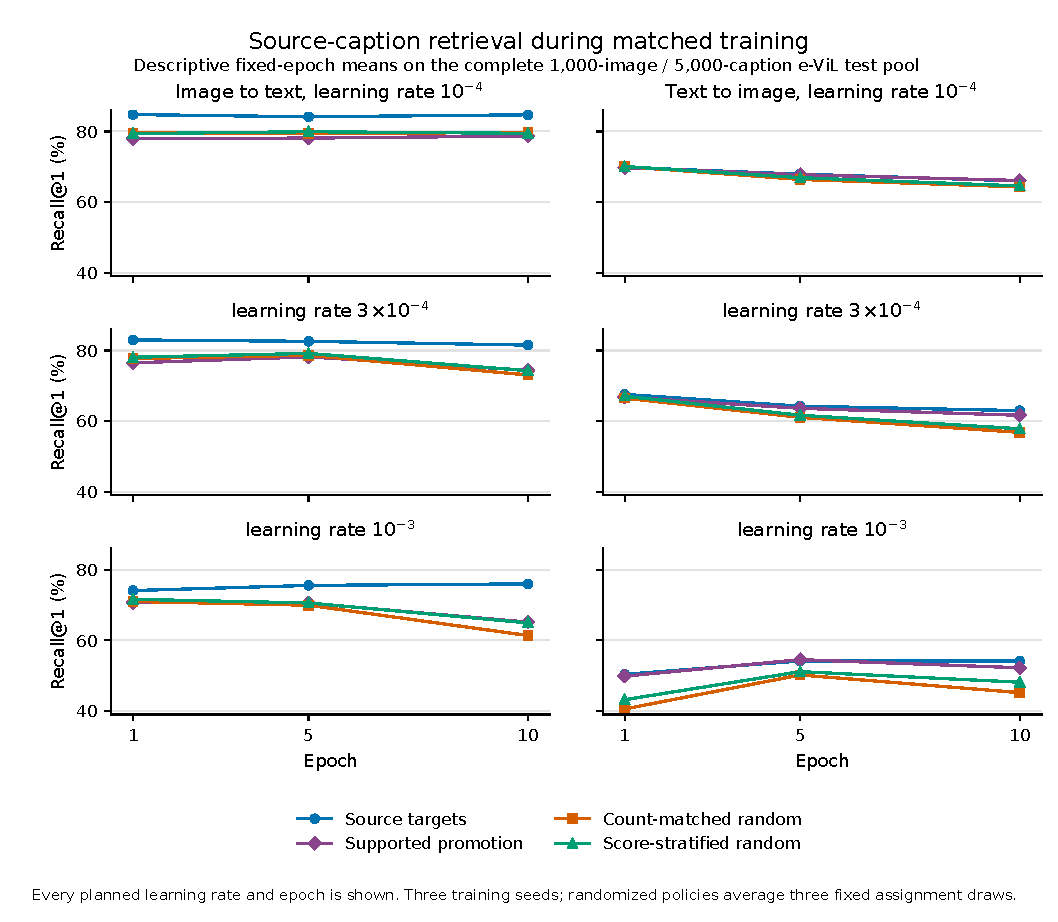
\includegraphics[width=\textwidth]{followup_trajectories.pdf}
\caption{Descriptive source-pool retrieval at epochs one, five, and ten. Every learning rate is displayed. Randomized families average all assignment draws equally within seed. The primary family concerns epoch ten only.}\label{fig:futrajectories}
\end{figure*}
